\chapter{Введение в программирование на Perl}
\section{История}
\subsection{Появление языка Perl}
18 декабря 1987г. — вышла первая версия языка программирования Perl, создан он был программистом Ларри Уоллом (Larry Wall). В названии этого языка кроется аббревиатура practical extraction and report language. Однако не сложно заметить, что в аббревиатуре не хватает одной буквы «a» (PEARL). Но затем стало известно, что такой язык существует, и букву «a» Ларри решил убрать, тем самым почти не изменив звичание. Символом языка Perl является верблюд — не слишком красивое, но очень выносливое животное, способное выполнять тяжёлую работу.

Целью Ларри Уолла никогда не было получение денег. Напротив, он внёс существенный вклад в культуру бесплатного распространения программ с их исходными кодами как средств работы программистов. Новый язык программирования Уолл разрабатывал для того, чтобы решить проблемы программистов, с которыми он сам сталкивался в течение рабочего дня. Когда первая версия языка вышла в свет, Ларри Уолл обеспечил открытый доступ и к исходному коду самой программы. Любой желающий может бесплатно скачать и пользоваться Perl независимо от того, нужен ли он ему для усовершенствования собственной странички или для создания мультимилионного Интернет-проекта. 

Перл создавался в среде Unix, которая оказала существенное влияние на развитие языка и его популярность. Среда Unix изначально создавалась группой программистов для самих же себя — удобное рабочее место программиста. Перл перенял такие принципы как:
- максимально функционально
- кратко
- единообразно

\subsection{Становление языка Perl}
Благодаря языку Perl стартовал Yahoo — проект, авторам которого прекрасно удаётся заработок на сайте. С его же помощью создан Amazon и миллионы других сайтов.

Однако новому языку для обработки текстов было не просто. Как и упоминалось ранее, Perl стартовал в среде unix, а в ней уже существовали другие утилиты по обработке текста: awk, sed, grep и другие. Собственно, которые и стали толчком к появлению языка Perl. Perl включал в себя всё самое нужное из имеющихся на тот момент утилит и упрощал/ускорял работц системных администраторов, за что и полюбился огромному их числу.
Так же нельзя не отметить, что Perl был лёгок в изучении и применении, т.к. в большенстве случаев он повторял синтаксис других утилит. С его помощью действительно можно было решить большинство повседневных задач

\subsection{Развитие языка Perl}
Развитие на то время было мотивированно тем, что программисты из разных стран отправляли Ларри Уоллу предложения по модернизации языка и доработкам. Аудитория использования языка росла и её потребности тоже. 
\begin{itemize}
 \item 1988 году вышла версия 2.0
 \item1989 году вышла версия 3.0
 \item1991 году вышла версия 4.0
 \item1994 году появляется знаменитая 5 версия языка Perl
\end{itemize}
При её подготовке Ларри Уолл многое переосмыслил, и почти полностью переписал. Такие большие изменения были сделаны из-за того, что Ларри Уолл был не в состоянии принимать все доработки которые ему присылали, более того, и не успевал делать новые возможности. С этой версии Perl стал модульным в нем появились зачатки ООП
\verb|"Настоящее величие в том, сколько свободы вы даёте другим, а не в том, как вам удаётся заставлять других делать то, что вы хотите" - Ларри Уолл|
До выхода 5 версии Ларри делал Perl для сообщества и по просьбе сообщества. А начиная с версии 5.0 он стал придерживаться позиции, что теперь этот язык должно делать сообщество само для себя и под свои нужды. Что сыграло большой плюс в развитие языка для широкого применения, который следовал модным тенденциям, так и минус в том, что сам язык перестал выпускать новые версии.

До 2009 года было примерно 200 релизов 5 версии языка perl. Были даже параллельные разработки разных направлений развития языка. perl 5.005 развивался отдельно и параллельно вплоть до 2009 года. 
А вышедший в 2000 году перл версии 5.6.0 с поддержкой юникода вытеснил другие версии впитав в себя все полезное из них

На этом развитие языка не закончилось, Perl продолжает развиваться, в 2003 году появляется сайт perl6.ru

\verb|"Перл 5 уже начал умирать, потому что люди воспринимали его как тупиковый язык. Странно, но когда мы объявили Перл 6, Перл 5 неожиданно обрёл второе дыхание" - Ларри Уолл|

27 ноября 2004 года был выпущен релиз 5.8.6. В него включили все необходимое/недостающее для:
\begin{itemize}
 \item написания модулей
 \item работы с юникодом
 \item создания высокопроизводительных приложений
\end{itemize}

И с этого момента опять происходит изменение акцентов развития языка. Для большенства нужд Perl не требовал доработок вовсе. Все занялись написанием модулей, Сам Perl развивался неспешно, новые версии появлялись только, как тестовые, что бы оценить возможность внедрения новых фич или ускорение существующих, и не сломать функциональность и работоспособность большенства модулей.

Но Параллельно началась разработка perl 5.10, который впитывал в себя всё самое интересное из 6 версии.

В начале 2006 года вышла версия 5.8.8. Мотивирован выпуск этой версии был улучшениями для работы с XS модулями. В этот момент борьбы пошла не за удобство использования и универсальность, а за скорость. Так же в этот релиз вошло множество мелких исправлений, мешающих разработке новых модулей и программ.

\subsection{Perl 6}

Как уже упоминалось раннее сайт perl6.ru появился в 2003 году. Что то вменяемое и рабочее можно было написать только к 2010 году. В 2014 году стало все гораздо лучше, но в продакшене мы его еще не увидели. 25 декабря 2015 года состоялся релиз компилятора Rakudo 2015.12. И теперь можно присоединятся к немогочисленным разработчикам на perl6!

И как это не парадоксально, но perl6 сыграл очень большую роль в развитии perl5. Внедрение «современности», а именно полноценная поддержка классов была успешна реализована в perl5. Не один раз и не за один подход («Есть больше одного способа сделать это» и «Простые вещи должны оставаться простыми, а сложные — стать выполнимыми»).

\subsection{Утверждение языка}
Вернёмся немного назад язык Perl версии 5 с самого своего появления:
\begin{itemize}
 \item стал активно занимать нишу разработки WEB приложений
 \item укреплять свои позиции среди системных администраторов
 \item количество однострочников, написанных системными администраторами, всего мира не поддаётся исчислению
\end{itemize}

Однострочник: программа написанная в одной строке, как правило не более 200 символов.

В 2002 году Perl был исключён из стандартной поставки FreeBSD. Что еще в тот момент породило множество статей  о несостоятельности Perl-а и внесло смуту в рады системных администраторов. Однако обусловлено это было тем, что в стандартной поставке FreeBSD был perl версии 5.0, а в портах уже жил 5.6. Релиз инженеры FreeBSD не готовы были обновить версию Perl-а из-за того, что часть модулей не была способна работать с новой версией, а занимать актуализацией всех пакетов, а на тот момент их были сотни, было принято решение исключить вообще весь софт на Perl-е из поставки операционной системы и дать возможность системным администраторам самим выбрать нужную им версию с необходимыми модулями. Таким образом это неявно повлекло к обновлению версии Perl на множестве новых серверов. Системные администраторы выбирали более новую версию из-за того, что она была более безопастной в плане эксплуатации, а разработчики из-за того, что она была более функциональной.

До 2005 года perl занимал в нише web программирования лидирующее положения. Разработчики руководствовались тем, что PHP было мало, а Java была уже перебором выбор останавливался на Perl.

С 2005 года перл начал терять свои позиции в области веб разработки. Началом этого послужило давление со стороны PHP. Проигрыш языку, который создавался именно для web-разработки, был логичным. У языка Perl не было сравнимого по своим функциям IDE. Порог входа в PHP ниже и из-за этого стоимость разработчика на Perl была намного выше, чем на PHP. Ну и конечно же любимое в тот момент высказывание: \verb|Некрасивые ошибки вида "Internal Server Error"|

Примерно в конце 2006 года в сети Интернет стали встречаться посты «Perl умер». О Перле стали меньше говорить, но он продолжает делать свою работу. Опять таки из-за того, что не было выхода новых версий, небыло и статей, Perl на тот момент был известным языком со своим набором функций и большим кол-вом модулей, про это все уже знали и говорить об этом еще раз ни кто не хотел. Примерно в это же время появился Python 3.0, хипстеры качают новый язык, а он действительно во многом получился новым. Так же близился релиз второй версии ruby on rails. Ну и нельзя не отметить, что это высказывание было простимулированно долгим созданием 6 версии языка.

Он окунёмся в цифры:
\begin{itemize}
 \item В 2006 году было выпущено более 3000 модулей для perl
 \item В 2007 году приблизительно 5500 модулей
\end{itemize}

\begin{figure}[H] \centering
  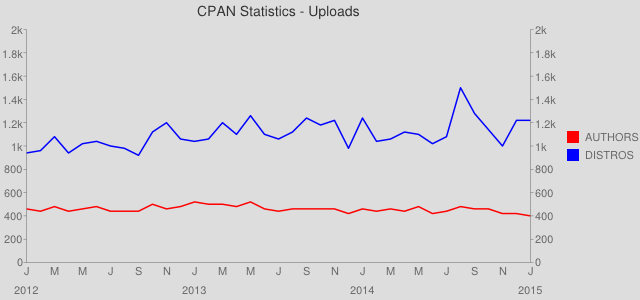
\includegraphics[width=10cm]{lectures/L1/stats6.png}
\end{figure}\noindent

К 2008 году по всему миру было собрано много групп Perl Mongers пытаясь противостоять вытеснению языка perl. В 2014 году их было примерно 256 групп, 8 из них в России. Эти цифры уже ушли в историю, но о их нельзя было не заметить.

\begin{figure}[H] \centering
  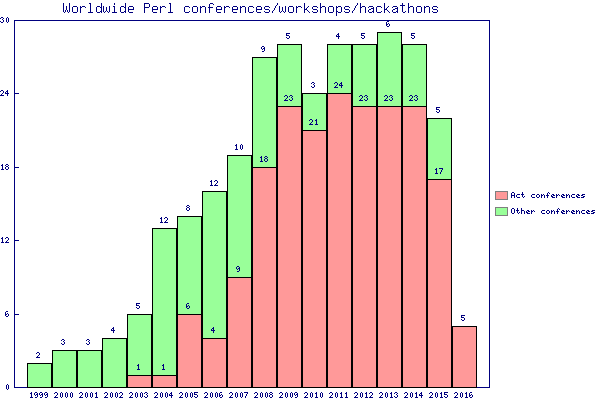
\includegraphics[width=10cm]{lectures/L1/act-conferences.png}
\end{figure}\noindent

\verb|act| - конференции программа которых зарегистрирована и размещена на официальном сайте Moungers групп.

На конференции O'Reilly's Money по финансовым технологиям в Нью-Йорке в 2008 году подсчитали количество упоминаний докладчиками базовых технологий.

Топ 3:
\begin{itemize}
 \item Перл
 \item SQL
 \item XML
\end{itemize}

И еще немного статистических данных:

На конец 2015 года было 600 000 уникальных посетителей CPAN в месяц. По грубым оценкам в мире на 1000 человек 1 программист ~6,5 миллионов программистов. Из этого можно примерно посчитать что 1 из 10-20 пишет на Perl. И не просто пишет, а заливает свои наработки в общую библиотеку модулей.


\subsection{Рынок труда}

Публикуемые вакансии:
\begin{figure}[H] \centering
  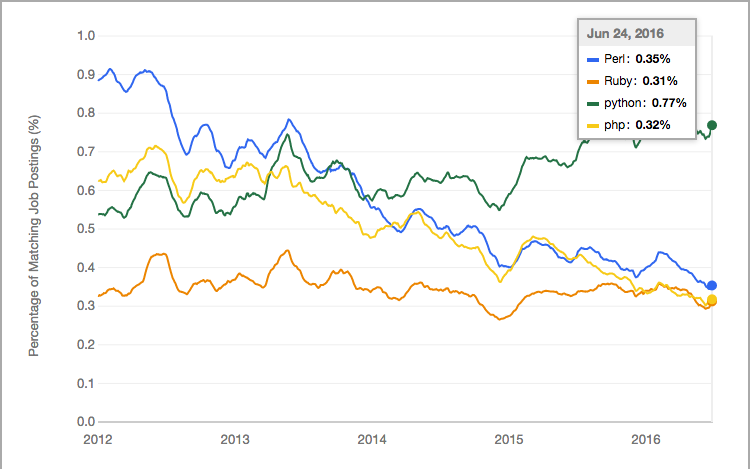
\includegraphics[width=10cm]{lectures/L1/jobgraph.png}
\end{figure}\noindent

Отношение публикуемых вакансий к соискателям:
\begin{figure}[H] \centering
  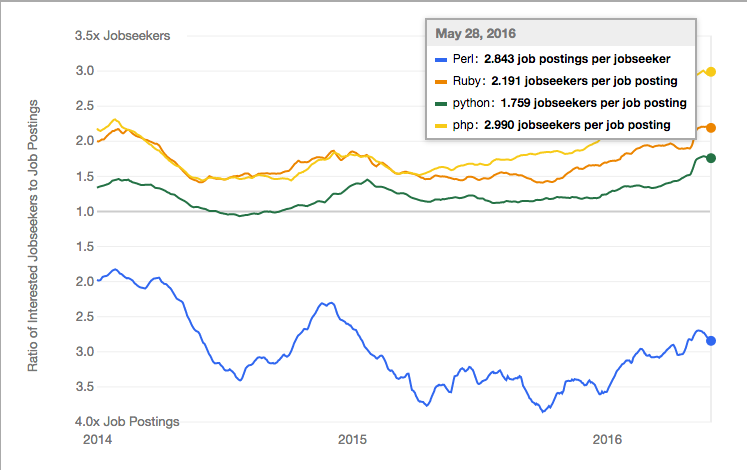
\includegraphics[width=10cm]{lectures/L1/jobgraph1.png}
\end{figure}\noindent

Зарплаты
\begin{figure}[H] \centering
  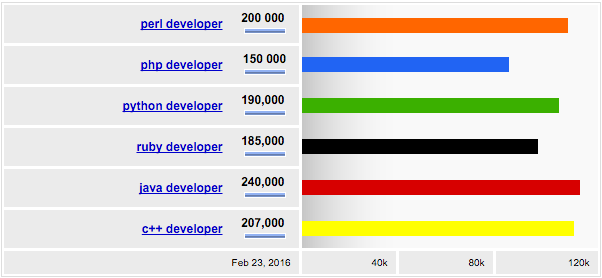
\includegraphics[width=10cm]{lectures/L1/zp.png}
\end{figure}\noindent

\subsection{Итог}
На сегодняшний день мы имеем:
\begin{itemize}
 \item  хорошо зарекомендовавший себя язык
 \item Огромную быстро растущую библиотеку
 \item Большое, активное сообщество
 \item Язык Perl6 и его отличный прототип, который вносит свои коррективы в развитие perl5
 \item идею сделать perl7, который быстро попадёт в продакшин, основываясь на опыте создания perl6 и надобности perl5
 \item Высокие зарплаты
\end{itemize}


\section{Настройка окружения}
\subsection{Настройка окружения в Mac OS}
Сам perl уже предустановлен (узнать версию можно, если набрать \verb|perl -v| в командной строке), но для сборки сторонних XS-модулей придётся установить xcode, <<Command line tools>>. Также, возможно, придется использовать macports (это perl установленный в отдельную директорию, отличный от системного).

Подробнее про установку можно прочитать в perldoc \perldoc{perlmacosx}.

\subsection{Настройка окружения в Linux}
Как правило перл есть в репозиториях дистрибутива. Команды для установки для некоторых дистрибутивов:
\begin{itemize}
 \item для CentOS: \verb|yum install perl| (Как правило в CentOS версия perl обновляется крайне редко. Поэтому, если необходима более современная версия, ее придется собирать самостоятельно.)
 \item для Debian: \verb|apt-get install perl|
 \item для GenToo: \verb|emerge dev-lang/perl|
 \item для FreeBSD: \verb|pkg add perl|
\end{itemize}
Сборки Perl есть почти под все операционные системы, даже под некоторые микроконтроллеры. Чтобы самостоятельно собрать perl, нужно скачать исходный код и выполнить:
\begin{minted}{bash}
make perl ./Configure -des; make test instal
\end{minted}
Если нужно установить его в другую директорию, нужно указать это с помощью ключей для make.

\subsection{Настройка окружения в Windows}
Для Windows существует несколько дистрибутивов Perl:
\begin{itemize}
  \item \textbf{ActivePerl от ActiveState}. Фирма ActiveState знаменита тем, что сделала Perl продакшн-системой, модули для которой они продавали.
  \item \textbf{StrawberryPerl} (рекомендуется использовать). В отличие от ActivePerl, StrawberryPerl идёт сразу с компилятором mingw, а также существенно удобнее и проще установка модулей.
  \item \textbf{cygwin}
\end{itemize}
С ActivePerl надо позаботится о наличие nmake + win32GnuUtils иначе сборка модулей будет мучительной и утомляющей.


\subsection{Проверка доступности интепретатора}
Чтобы проверить доступность интерпретатора, необходимо набрать в терминале:
\begin{minted}{bash}
  perl -v
\end{minted}
Выдача будет примерно такой:
\begin{minted}{bash}
This is perl 5, version 18, subversion 2 (v5.18.2) built for
x86_64-linux-gnu-thread-multi
(with 40 registered patches, see perl -V for more detail)

Copyright 1987-2013, Larry Wall

Perl may be copied only under the terms of either the Artistic License or the
GNU General Public License, which may be found in the Perl 5 source kit.

Complete documentation for Perl, including FAQ lists, should be found on
this system using "man perl" or "perldoc perl".  If you have access to the
Internet, point your browser at http://www.perl.org/, the Perl Home Page.
\end{minted}

Если вместо этого выводится ошибка <<Command not found>> или какая-то другая, то с установкой, что то пошло не так. Возможно, интерпретатор находится за пределами возможных путей из переменной окружения среды PATH.

\section{Базовый синтаксис языка Perl}
Синтаксис языка Perl близок к синтаксису языка C, а также в нем реализованы идеи и конструкции из shell, awk (популярная утилита для работы с табличными данными), sed и так далее.

\subsection{Простые конструкции в Perl}
Каждая программа на Perl представляет собой последовательность утверждений (statement). Комментарии в языке Perl начинаются с символа \verb|#|.
\begin{minted}{perl}
$a = 42;
say "test";
eval { ... };
do { ... };
my $var;
# Комментарий
\end{minted}
Каждое утверждение возвращает некоторое значение.
\begin{minted}{perl}
# Простые конструкции возвращают значение
$a = 42;        # => 42
say "test";     # => 1
eval { 7 };     # => 7
do { 1; 2; 3 }; # => 3
my $var;        # => undef
\end{minted}
Если утверждение --- это вызов функции, то возвращается значение, которое было возвращено функцией. Если утверждение --- это присвоение переменной некоторого значения, то возвращается значение этой переменной.

\subsection{Инициализация переменных. Режим strict}
Следует отметить, что Perl --- нетипизированный язык, любой переменной можно присвоить значение любого типа. Одна и та же переменная в различных участках программы может принимать значения разных типов.

Одна из особенностей Perl заключается в том, что новые переменные инициализируются автоматически в момент первого использования. Это было очень удобно для создания программ-однострочников, но создавало массу проблем в крупных проектах, когда при опечатке в имени какой-либо переменной Perl просто создавал еще одну переменную при этом менялась логика работы программы, но ошибка оставалась незамеченной и найти её было крайне сложно.

Поэтому в Perl появилась специальная директива strict, которая включает так называемый строгий режим. В этом режиме все переменные должны быть явно инициализированы до их первого использования. В ином случае на этапе компиляции кода выводится исключение о том, что была попытка использовать не объявленную переменную. Инициализация переменной происходит с помощью функции my. Хорошим тоном считается писать все программы (длиной более строчки) в режиме strict.

\subsection{Блоки. Область видимости переменной}
Блоком (scope) называется все, что заключено в фигурные скобки:
\begin{minted}{perl}
{
statement;
statement;
...
}
\end{minted}
Переменные, объявленные внутри такого блока, не видны за его пределами. Это свойство позволяет локализовывать части кода.


\subsection{Управляющие конструкции}
В Perl доступны следующие управляющие конструкции:
\begin{itemize}
  \item \textbf{Условия:} \verb|if|, \verb|unless|, \verb|elsif|, \verb|else|
  \begin{minted}{perl}
    if     ( EXPR ) { ... }
    elsif  ( EXPR ) { ... }
    else            { ... }
  \end{minted}
  С помощью \verb|else| и \verb|elsif| (именно так, а НЕ \verb|elseif| или \verb|else if|) можно указать, что должно быть выполнено, если условие не выполнено. Команда \verb|elsif|, в отличие от \verb|else|, сначала проверяет другое условие. Если условие выполняется, то исполняется код в фигурных скобках, а в ином случае программа переходит к следующему \verb|elsif| или  \verb|else|, если они есть.

  Такой же синтаксис и у команды \verb|unless|:
  \begin{minted}{perl}
      unless ( EXPR ) { ... }
  \end{minted}
  В этом случае код в фигурных скобках выполняется только, если выполнено условие в круглых скобках. При этом плохим тоном считается использование конструкций такого вида:
  \begin{minted}{perl}
      unless ( EXPR ) { ... }
      elsif  ( EXPR ) { ... }
      else            { ... }
  \end{minted}

  \item \textbf{Циклы:} \verb|while|, \verb|until|, \verb|for|, \verb|foreach|
  \begin{minted}{perl}
  while ( EXPR ) { ... }
  \end{minted}
  Оператор \verb|while| исполняет код в теле цикла, пока выполнено некоторое условие. Использование ключевого слова \verb|continue| позволяет указать блок кода, который будет выполнен всегда после каждой итерации. Например, если был совершен преждевременный выход из цикла, блок \verb|continue| все равно будет выполнен. Оператор \verb|until| имеет похожий синтаксис, но выполняет код в теле цикла, пока условие не выполнено:
  \begin{minted}{perl}
  until ( EXPR ) { ... } continue { ... }
  \end{minted}
  Еще два оператора for и foreach являются синонимами в Perl и позволяют итерировать по значениям целочисленной переменной и по элементам списка:
  \begin{minted}{perl}
  for ( EXPR; EXPR; EXPR ) { ... }
  for ( LIST ) { ... }
  for VAR ( LIST ) { ... } # Объявляется переменная, которая будет доступна в обоих scope.
  for VAR ( LIST ) { ... } continue { ... }
  \end{minted}
  \item \textbf{Выбор:} \verb|given|, \verb|when|
  \item \textbf{Безусловный переход:}  \verb|goto|
\end{itemize}

\subsection{Типы данных в Perl}
Основные типы данных в Perl включают в себя:
\begin{itemize}
  \item \textbf{SCALAR}~--- простая переменная, имя всегда начинается с символа \verb|$|, может содержать одно из следующих значений:
  \begin{itemize}
    \item \textbf{Number} (числовое значение): \verb|$s = 1|, \verb|$s = -1e30|.
      Perl работает с числовыми значениями как с числами (то есть быстро) до тех пор, пока не будет к ним обращения как к строке. В последнем случае числовое значение будет преобразовано в строковое.

    \item \textbf{String} (строковое значение): \verb|$s = "str"|. Строка в Perl всегда обрамлена в кавычки.
    \item \textbf{Reference} (ссылка): разыменовывание ссылки \verb|$r| делается в зависимости от того типа данных, который предпологается, что лежит по ссылке:
      \begin{itemize}
        \item \textbf{Scalar} (\verb|$$r|, \verb|${ $r }|)
        \item \textbf{Array} (\verb|@$r|, \verb|@{ $r }|, \verb|$r->[...]|)
        \item \textbf{Hash} (\verb|%$r|, \verb|%{ $r }|, \verb|$r->{...}|)
        \item \textbf{Function} (\verb|&$r|, \verb|&{$r}|, \verb|$r->(...)|)
        \item \textbf{Filehandle} (\verb|*$r|)
        \item \textbf{Lvalue} (\verb|$$r|, \verb|${ $r }|)
        \item \textbf{Reference} (\verb|$$r|, \verb|${ $r }|)
      \end{itemize}
    Нужно иметь в виду, что, если разыменовать ссылку на хэш как массив, получится каша, а именно: получится массив из поочередно ключей и соответствующих значений.
  \end{itemize}
  \item \textbf{ARRAY} (\verb|@a|, \verb|$a[...]|)
  \item \textbf{HASH} (\verb|%h|, \verb|$h{key}|, \verb|$h{...}|)
\end{itemize}


\subsection{Специальные переменные}
В perl существуют специальные глобальные переменные, которые позволяют существенно упростить написание программ:
\begin{itemize}
  \item \verb|$_|, \verb|$ARG| --- аргумент по умолчанию,
  \item \verb|@_|, \verb|@ARG| --- аргументы функции (как массив).
  \item \verb|$a|, \verb|$b| --- переменные, используемые при сортировке:
  \begin{minted}{perl}
  for (sort { $a <=> $b } @ARGV) {
  say "Arg: $_";
  }
  say "Was run by $ENV{USER}";
  \end{minted}
  Поэтому при написании программы категорически не рекомендуется заводить переменные с такими же именами.
  \item \verb|%ENV| --- переменные окружения (как хэш),
  \item \verb|@ARGV| --- аргументы программы (как массив).
\end{itemize}
Также существуют следующие специальные переменные:
\begin{itemize}
  \item \verb|$"|, \verb|$LIST_SEPARATOR| --- разделитель при интерполяции в кавычках.
  \item \verb|$,|, \verb|$OUTPUT_FIELD_SEPARATOR| --- разделитель между элементами списка при выводе (при выводе на экран массива его элементы будут разделены этим символом)
  \item \verb|$/|, \verb|$INPUT_RECORD_SEPARATOR| --- разделитель входного потока для readline
  \item \verb|$\|, \verb|$OUTPUT_RECORD_SEPARATOR| --- разделитель выходного потока для print
  \item \verb|$.|, \verb|$INPUT_LINE_NUMBER|
\end{itemize}
Пример использования:
\begin{minted}{perl}
$" = "."; # $LIST_SEPARATOR
$, = ";"; # $OUTPUT_FIELD_SEPARATOR
$\ = "\n\n"; # $OUTPUT_RECORD_SEPARATOR
while (<>) {
    chomp;
    @a = split /\s+/, $_;
    say "$. @a",@a;
    }
\end{minted}
Есть еще ряд специальных переменных:
\begin{itemize}
  \item \verb|$!|,  \verb|ERRNO|~--- переменная в которую записываются ошибки при открытии файлов.
  \item \verb|$<|,  \verb|UID|~--- ID пользователя, запустившего программу.
  \item \verb|$$|,  \verb|PID|~--- PID процесса
  \item \verb|$0|,  \verb|PROGRAM_NAME|~--- Имя программы
  \item \verb|$^X|,  \verb|EXECUTABLE_NAME|~--- название запущенного бинарного файла
  \item \verb|$^O|,  \verb|OSNAME|~--- имя используемой операционной системы
  \item \verb|$^V|,  \verb|PERL_VERSION|~--- версия perl
\end{itemize}

Например:
\begin{minted}{perl}
say "I'm $^X, $^V, on $^O";
say "Script: $0 (@ARGV);";
say "Pid $$ by uid $<";
open my $f, '<','/etc/shadow'
or die "No shadow: $!\n";
\end{minted}

\begin{minted}{bash}
/usr/bin/perl sample.pl -test
\end{minted}

\begin{verbatim}
# I'm /usr/bin/perl, v5.18.2, on darwin
# Script: sample.pl (-test);
# Pid 70032 by uid 502
# No shadow: No such file or directory
\end{verbatim}

\section{Запуск однострочных скриптов}
Perl в начале своего развития использовался для запуска и исполнения простейших однострочных скриптов. Также, за исключением небольшого числа системнозависимых библиотек, Perl на всех операционных системах работает одинаково. Именно поэтому Perl был так популярен среди системных администраторов.

При написании однострочников \verb|use strict;| писать необязательно. Но если вдруг скрипт начал выполнять не то, что задумано, лучше добавить \verb|use strict;|, что упростит отладку.

Запустить однострочник можно с помощью ключа \verb|-e|, после которого идет код однострочника в кавычках:
\begin{minted}{bash}
perl -e 'print "Hello world\n"'
\end{minted}
Использовать всегда следует одинарные кавычки, так как разные шеллы по-разному работают с двойными кавычками, и существует соглашение, что одинарные кавычки --- неинтерполируемые (то есть в них не будут подставляться переменные среды). Обычно однострочная программа, обрабатывает данные приходящие ей в стандартном вводе. Вот простейшая программа которая читает стандартный ввод и распечатывает строки добавляя в начало каждой из них дефис
\begin{minted}{bash}
perl -e 'while(<>){print "- ".$_}'
\end{minted}
Чтобы постоянно не использовать конструкцию \verb|while(<>){}| при выполнении действия над каждой строчкой в файле, существует ключ \verb|-n|. Идентичная запись той же программы:
\begin{minted}{bash}
perl -ne 'print "- ".$_'
\end{minted}
Внутри цикла \verb|while(<>){}| переменная \verb|$_| будет содержать цельную строку вместе с символом \verb|\n|. Что бы не использовать команду chomp (отрезающую в конце перенос строки) можно использовать флаг \verb|-l|, который:
\begin{itemize}
  \item устанавливает переменную \verb|$\| (разделитель, который выведен после каждого выполнения команды print)
  \item устанавливает переменную \verb|$/| (разделитель по которому будет делится входящий поток, отдельно его можно выставить с помощью флага \verb|-0|)
  \item удаляет из строки \verb|$_| последний перенос строки (при совместном использовании с флагом \verb|-n|)
\end{itemize}
Например, прочитать файл в котором записи разделены через \verb|";"| и вывести каждую запись на новой строке можно так:
\begin{minted}{bash}
perl -nl00120073 -e 'print $_'
\end{minted}
Все строки из файла записать через \verb|";"| можно так:
\begin{minted}{bash}
perl -nl00730012 -e 'print $_'
\end{minted}
Флаг \verb|-p| делает тоже самое, что и флаг \verb|-n|, только в каждую итерацию цикла добавит еще вывод переменной \verb|$_|:
\begin{minted}{bash}
perl -nl00120073 -e ''
\end{minted}
\begin{minted}{bash}
perl -pl00730012 -e ''
\end{minted}
Детальнее можно посмотреть тут: perldoc \perldoc{perlvar}.

Для парсинга более сложных структур файлов (например, когда в каждой строке есть записи разделенные определённым разделителем), можно использовать флаг  \verb|-a| совместно с \verb|-F|:
\begin{itemize}
  \item Флаг \verb|-a| добавляет функцию разделяющую входную строку на части и складывает в спецмассив \verb|@F|
  \item \verb|-F| устанавливает разделитель (по умолчанию это пробел)
\end{itemize}
Например, с помощью следующего кода можно прочитать файл-таблицу, в которой каждая строка представляет собой набор полей разделенных \verb|";"|, проверить третью колонку на наличие там 1 и при выполнении условия вывести значение из 2 колонки:
\begin{minted}{perl}
perl -lnaF';' -e 'if( $F[2] == 1 ){ print $F[1] };'
\end{minted}
В этом примере флаг \verb|-l| необходим, чтобы выполнять скрипт для каждой строки файла.

\subsection{Система CPAN}
Perl завоевал к себе доверие, за счет того, что был портирован под всевозможные платформы и системы, а также за счет большой системы CPAN. CPAN --- архив модулей, написанных на языке программирования Perl.
Все версии модулей под все версии perl проходят тестирование (разработчик модуля должен сам должен предоставить тесты) автоматической системой на CPAN. Эта система запускает модуль на каждой версии perl и отмечает результат выполнения тестов в специальной таблице. Часто при крупных обновлениях perl некоторые модули перестают работать, поэтому при выборе модуля для работы эта таблица может оказаться полезной.

\begin{figure}[H] \centering
  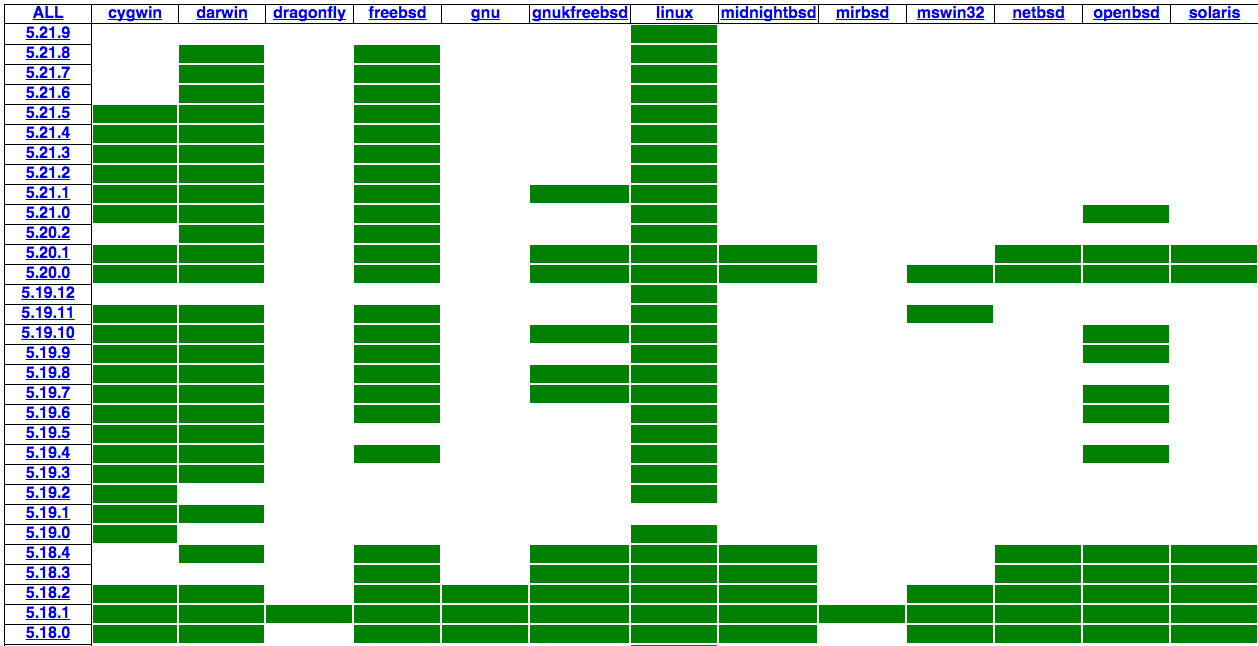
\includegraphics[width=10cm]{lectures/L1/matrixcpantesters.png}
\end{figure}\noindent

Подключить модули (чтобы иметь возможность пользоваться функциями этого модуля) можно опцией \verb|-M|, например:
\begin{minted}{perl}
perl -MJSON::XS -e 'print JSON::XS::encode_json({var1 => 1, var2 => 2})'
\end{minted}
Perl поддерживает еще много других ключей, но представленных должно быть достаточно для начала изучения языка.

\section{Средства отладки в Perl}
\subsection{Доступ к кодам операции}
В perl 5 (начиная с версии 5.005) был обеспечен доступ к компилятору. По умолчанию Perl переводит исходный код в коды операции и исполняет их. Если вы не хотите выполнять свою программу, а хотите проанализировать коды операции, то можно написать собственный модуль или воспользоваться существующим. Для таких модулей было выделено пространство имен \verb|B::|). Доступ к компилятору организован, через модуль \verb|O|, таким образом для передачи кодов операций в некоторый модуль для их анализа, следует использовать модуль \verb|O|, передавая ему имя модуля для получения кодов операций:
\begin{minted}{perl}
perl -MO=Backend
\end{minted}
Указанный модуль может вывести коды операций на экран, проанализировать быстродействие. Эта функция будет особенно полезна при отладке. Например, \verb|B::Concise| --- модуль, позволяющий вывести коды операции как есть.

\subsection{Модуль Deparse}
\verb|B::Deparse| --- модуль, который превращает коды операции после компилятора обратно в код на perl, то есть декомпилирует коды операций. У этого модуля есть множество опций, позволяющих менять его поведение.

Работу модуля можно продемонстрировать на программе
\begin{minted}{perl}
perl -pl00730012 -e ''
\end{minted}
запуская perl с подключенным модулем B::Deparse:
\begin{minted}{perl}
perl -MO=Deparse -pl00730012 -e ''
\end{minted}
На выходе получается:
\begin{minted}{perl}
BEGIN { $/ = "\n"; $\ = ";"; }
LINE: while (defined($_ = <argv>) ){
    chomp $_;
}
continue {
    die "-p destination: $!\n" unless print $_;
}
-e syntax OK
\end{minted}
У модуля B::Deparse есть свои удобные ключи:
\begin{itemize}
  \item \verb|-l| добавит комментарии с ссылками на строки исходного файла
  \item \verb|-p| расставит скобки и тем самым покажет приоритетность выполнения команд
  \item \verb|-q| развернёт интерполируемые строки, то есть представит их как конкатенацию неинтерполируемых строк и переменных. Интерполирование строк --- это поиск внутри строчек, которые обрамлены в двойные кавычки, имен переменных и замена их на соответствующие им значения:
  \begin{minted}{perl}
  "Hello $name" = 'Hello ' . $name != 'Hello $name'
  \end{minted}
  Строки в одинарных кавычках не интерполируются.
  \item Ключ \verb|-sС| определяет стиль вывода кода.
  \item Ключ \verb|-siNUMBER| определяет количество пробелов в отступе
  \item Ключ \verb|-siT| позволяет использовать символ табуляции
  \item Ключ \verb|-xNUMBER| определяет уровень развертывания кода
\end{itemize}
\verb|B::Deparse| можно использовать, как обычный модуль, передавая ему ссылку на функцию, код которой хочется посмотреть (в том числе, если доступна только ссылка на функцию):
\begin{minted}{perl}
use B::Deparse;
sub func {
    print 'Hello world!!!'
};

my $deparse = B::Deparse->new("-p", "-sC");
$body = $deparse->coderef2text(\&func);

print $body;
\end{minted}
После выполнения такой программы:
\begin{minted}{perl}
{
print('Hello world!!!');
}
\end{minted}

При уровне отладки большем чем 3 все циклы for будут развёрнуты в while. Код:
\begin{minted}{bash}
perl -MO=Deparse,x3 -e 'for ($i = 0; $i < 10; ++$i) {print $i;}'
\end{minted}
Превратится в
\begin{minted}{perl}
$i = 0;
while ($i < 10) {
    print $i;
} continue {
    ++$i
}
\end{minted}
\subsection{Data::Dumper}
\verb|Data::Dumper| - модуль, который поможет выводить на экран в развернутом виде сложные структуры данных. Например:
\begin{minted}{perl}
use Data::Dumper;
my $foo = [{a => 1, b => 2},{c => 3, d => 4}];
print Dumper($foo);
\end{minted}
Вот так красиво демонстрирует эту переменную \verb|Data::Dumper|:
\begin{minted}{perl}
$VAR1 = [
    {
      'b' => 2,
      'a' => 1
    },
    {
      'c' => 3,
      'd' => 4
    }
];
\end{minted}
У \verb|Data::Dumper| есть множество опций, которые позволяют управлять стилем вывода: табуляцией, переносом строк и так далее.

\subsection{Модуль DDP (Data::Printer)}
Есть альтернативный модуль для просмотра структур и объектов. Его обычно используют для отладки приложений. У этого модуля не меньше настроек, чем у Data::Dumper, но его проще использовать, например:
\begin{minted}{perl}
use DDP;
my $foo = {a=>1, b=> 2, c=> [1,2,3]};
p $foo;
\end{minted}
Вывод следующий:
\begin{minted}{perl}
\ {
    a   1,
    b   2,
    c   [
        [0] 1,
        [1] 2,
        [2] 3
    ]
}
\end{minted}
Модуль DDP в основном отличается от Data::Dumper следующим:
\begin{itemize}
  \item Автор этого модуля позаботился о цветовой разметке выводимых данных, для удобства чтения.
  \item Так же у этого модуля более расширенный дамп объектов:
  \begin{minted}{perl}
  \ SomeClass  {
    Parents       Moose::Object
    Linear @ISA   SomeClass, Moose::Object
    public methods (3) : bar, foo, meta
    private methods (0)
    internals: {
      _something => 42,
    }
  }
  \end{minted}
  \item Отсутствует сериализация.
\end{itemize}

\subsection{Использование отладчика}
Для начала работы с дебагером рекомендуется прочитать документацию \perldoc{perldebtut}. Отладка программ подразумевает построчное их выполнение с возможностью просмотра состояния переменных между ними.

Запуск отладчика выполняется добавлением ключа \verb|-d| при запуске интерпретатора:
\begin{minted}{perl}
perl -d myscript.pl
\end{minted}
Для того, что бы отладчик запустился скрипт не должен содержать синтаксических ошибок и должен нормально компилироваться через \verb|perl -c|. После запуска отладчика на экране появится:
\begin{minted}{bash}
Loading DB routines from perl5db.pl version 1.44
Editor support available.

Enter h or 'h h' for help, or 'perldoc perldebug' for more help.

DB<1>
\end{minted}
Далее отладчик ждёт команд. Некоторые команды отладчика для просмотра кода и значения переменных:
\begin{verbatim}
- l посмотреть код. Параметра можно указать номер строки, номер строки + интервал, диапазон строк, название функции. На выход вы получаете запрошенный код
- - посмотреть предыдущий код относительно текущей строки
- v посмотреть код вокруг указанной строки
- / поиск по коду в прямом направлении на вход эта команда принимает регулярное выражение, если ничего не передавать то отладчик продолжит поиск по предыдущему запросу
- ? поиск по коду в обратном направлении
- f загрузка файла для просмотра, на вход принимает имя файла
- . вернуть указатель на текущую позицию выполнения кода
- m $obj показать все методы объекта
- M показать список всех загруженных модулей
- S список всех доступных функций в данной точке
- [X|V] [Package] [str|~re] список переменных. Можно передать имя пакета внутри которого интересуют переменные, название переменно или регулярное выражение для названия переменной
\end{verbatim}
Команды отладчика для выполнения кода:
\begin{verbatim}
- p выполнить перл выражение и показать результат
- n шаг вперёд без захода в процедуру
- s шаг вперёд с заходом в процедуру
- T стек вызовов в данной точке
- ! повторить предыдущую команду. На вход можно передать номер команды в истории которую надо повторить
- source file - выполнить команды из файла
- с продолжить выполнение программы. Если параметром указать номер строки или имя функции, то отладчик продолжит выполнение до указанного места
- r продолжить выполнение скрипта до выхода из подпрограммы
- q выход из отладчика
\end{verbatim}
Точки останова, действия, точки наблюдения
\begin{verbatim}
- b < line|sub > [условие] - установить точку останова на указанную строку или функцию при выполнении условия
- B < ln|* > - снять точку останова
- a строка действие [условие] - установить действие которое сработает достигнув определённой строки
- A < line|* > - удалить действие
- w $var - установить наблюдение за переменной
- W $var|* - снять наблюдение за переменной
- L [a|b|w] - вывести список точек останова, действий, наблюдений за переменными
- R - начать скрипт заново оставив все точки останова, действия, наблюдения
\end{verbatim}

\subsection{Использование отладчика: пример}
В качестве примера будет показана отладка следующего скрипта:
\begin{minted}{perl}
use strict;

my $ret = 0;

foreach ( my $i = 0 ; $i < 50 ; $i++ ) {
    if ( $ret > $i ) {
        $ret -= $i;
    }
    else {
        $ret += $i;
    }
}
print $ret;
\end{minted}
Запуск отладки:
\begin{minted}{bash}
perl -d mydebug.pl
\end{minted}
Отладчик запустился и выдал приглашение:
\begin{minted}{bash}
Loading DB routines from perl5db.pl version 1.44
Editor support available.

Enter h or 'h h' for help, or 'perldoc perldebug' for more help.

main::(mydebug.pl:3):   my $ret = 0;

DB< 1 >
\end{minted}
Команда \verb|l| позволяет просмотреть код с указанием текущей позиции:
\begin{minted}{perl}
3==>    my $ret = 0;
4:      my $cnt_add = 0;
5:      my $cnt_sub = 0;
6
7:      foreach(my $i = 0; $i < 50; $i++){
8:              if($ret>$i){
9:                      $ret -= $i;
10              }
11              else {
12:                     $ret += $i;
\end{minted}
Установка точки останова (команда \verb|b|) на 8ой строчке при достижении 10 итерации цикла:
\begin{minted}{bash}
b 8 $i == 9
\end{minted}
Запуск программы (команда \verb|c|)
\begin{minted}{bash}
c
\end{minted}
Когда выполнится условие \verb|$i == 9|, сработает точка останова и на экране появится сообщение:
\begin{minted}{bash}
DB< 7 >
c
main::(mydebug.pl:8):           if($ret > $i){
\end{minted}
Вывод значения переменной \verb|$i|:
\begin{minted}{bash}
DB< 7 > print $i
9
\end{minted}
Отслеживать переменные можно командой \verb|$w|:
\begin{minted}{bash}
w $ret
\end{minted}
После этого выполнив 1 строчку (команда \verb|n|):
\begin{minted}{bash}
DB< 9 >
n
Watchpoint 0:   $ret changed:
old value:  ''
new value:  '16'
main::(mydebug.pl:9):                   $ret -= $i;

DB< 9 >
\end{minted}
Дальнейшая отладка происходит по тем же принципам.
